\documentclass[12pt]{article}

\usepackage{amsmath, mathtools}
\usepackage{amsfonts}
\usepackage{amssymb}
\usepackage{graphicx}
\usepackage{colortbl}
\usepackage{xr}
\usepackage{hyperref}
\usepackage{longtable}
\usepackage{xfrac}
\usepackage{tabularx}
\usepackage{float}
\usepackage{siunitx}
\usepackage{booktabs}
\usepackage{caption}
\usepackage{pdflscape}
\usepackage{afterpage}

\usepackage[round]{natbib}

%\usepackage{refcheck}

\hypersetup{
    bookmarks=true,         % show bookmarks bar?
      colorlinks=true,       % false: boxed links; true: colored links
    linkcolor=red,          % color of internal links (change box color with linkbordercolor)
    citecolor=blue,        % color of links to bibliography
    filecolor=magenta,      % color of file links
    urlcolor=cyan           % color of external links
}

%% Comments

\usepackage{color}

\newif\ifcomments\commentstrue

\ifcomments
\newcommand{\authornote}[3]{\textcolor{#1}{[#3 ---#2]}}
\newcommand{\todo}[1]{\textcolor{red}{[TODO: #1]}}
\else
\newcommand{\authornote}[3]{}
\newcommand{\todo}[1]{}
\fi

\newcommand{\wss}[1]{\authornote{blue}{SS}{#1}} 
\newcommand{\plt}[1]{\authornote{magenta}{TPLT}{#1}} %For explanation of the template
\newcommand{\an}[1]{\authornote{cyan}{Author}{#1}}

%% Common Parts

\newcommand{\progname}{ProgName} % PUT YOUR PROGRAM NAME HERE %Every program
                                % should have a name


% For easy change of table widths
\newcommand{\colZwidth}{1.0\textwidth}
\newcommand{\colAwidth}{0.13\textwidth}
\newcommand{\colBwidth}{0.82\textwidth}
\newcommand{\colCwidth}{0.1\textwidth}
\newcommand{\colDwidth}{0.05\textwidth}
\newcommand{\colEwidth}{0.8\textwidth}
\newcommand{\colFwidth}{0.17\textwidth}
\newcommand{\colGwidth}{0.5\textwidth}
\newcommand{\colHwidth}{0.28\textwidth}

% Used so that cross-references have a meaningful prefix
\newcounter{defnum} %Definition Number
\newcommand{\dthedefnum}{GD\thedefnum}
\newcommand{\dref}[1]{GD\ref{#1}}
\newcounter{datadefnum} %Datadefinition Number
\newcommand{\ddthedatadefnum}{DD\thedatadefnum}
\newcommand{\ddref}[1]{DD\ref{#1}}
\newcounter{theorynum} %Theory Number
\newcommand{\tthetheorynum}{T\thetheorynum}
\newcommand{\tref}[1]{T\ref{#1}}
\newcounter{tablenum} %Table Number
\newcommand{\tbthetablenum}{T\thetablenum}
\newcommand{\tbref}[1]{TB\ref{#1}}
\newcounter{assumpnum} %Assumption Number
\newcommand{\atheassumpnum}{P\theassumpnum}
\newcommand{\aref}[1]{A\ref{#1}}
\newcounter{goalnum} %Goal Number
\newcommand{\gthegoalnum}{P\thegoalnum}
\newcommand{\gsref}[1]{GS\ref{#1}}
\newcounter{instnum} %Instance Number
\newcommand{\itheinstnum}{IM\theinstnum}
\newcommand{\iref}[1]{IM\ref{#1}}
\newcounter{reqnum} %Requirement Number
\newcommand{\rthereqnum}{P\thereqnum}
\newcounter{nonreqnum} %Nonfunctionalrequirement Number
\newcommand{\rthenonreqnum}{P\thenonreqnum}
\newcommand{\rref}[1]{R\ref{#1}}
\newcounter{lcnum} %Likely change number
\newcommand{\lthelcnum}{LC\thelcnum}
\newcommand{\lcref}[1]{LC\ref{#1}}
\newcounter{ucnum} %Unlikely change number
\newcommand{\ltheucnum}{UC\theucnum}
\newcommand{\ucref}[1]{UC\ref{#1}}

\usepackage{fullpage}

\begin{document}

\title{Software Requirements Specification for Truss} 
\author{Ting-Yu Wu}
\date{\today}
	
\maketitle

\section*{Revision History}

\begin{tabularx}{\textwidth}{p{3.5cm}p{2cm}X}
	\toprule {\bf Date} & {\bf Version} & {\bf Notes}\\
	\midrule
	October 8, 2020 & 1.0 & Initial version of SRS\\
	November 16, 2020 & 2.0 & Modification according to feedback\\
	\bottomrule
\end{tabularx}

~\newpage

\pagenumbering{roman}

\tableofcontents

~\newpage

\section{Reference Material}

This section records information for easy reference.

\subsection{Table of Units}

Throughout this document SI (Syst\`{e}me International d'Unit\'{e}s) is employed
as the unit system.  In addition to the basic units, several derived units are
used as described below.  For each unit, the symbol is given followed by a
description of the unit and the SI name.
~\newline

\renewcommand{\arraystretch}{1.2}
%\begin{table}[ht]
  \noindent \begin{tabular}{l l l} 
    \toprule		
    \textbf{symbol} & \textbf{unit} & \textbf{SI}\\
    \midrule 
    \si{\metre} & length & metre\\
    \si{\radian} & angle & radian\\
    \si{\newton} & force & newton\\
    \bottomrule
  \end{tabular}
  %	\caption{Provide a caption}
%\end{table}

\subsection{Table of Symbols}

The table that follows summarizes the symbols used in this document along with
their units. The symbols are listed in alphabetical order.

\renewcommand{\arraystretch}{1.2}
%\noindent \begin{tabularx}{1.0\textwidth}{l l X}
\noindent \begin{longtable*}{l l p{12cm}} \toprule
\textbf{symbol} & \textbf{unit} & \textbf{description}\\
\midrule 
$d_{\text{max}}$ & \si{\metre} & Maximum value for distance \\
$d_{\text{min}}$ & \si{\metre} & Minimum value for distance \\
$F_\text{Ax}$ & \si{\newton} & x-component of reaction force on joint A \\
$F_\text{Ay}$ & \si{\newton} & y-component of reaction force on joint A \\ 
$F_\text{By}$ & \si{\newton} & y-component of reaction force on joint B \\
$F_\text{AC}$ & \si{\newton} & Force on truss member 1 \\
$F_\text{BC}$ & \si{\newton} & Force on truss member 2 \\
$F_\text{AD}$ & \si{\newton} & Force on truss member 3 \\
$F_\text{BD}$ & \si{\newton} & Force on truss member 4 \\
$F_\text{CD}$ & \si{\newton} & Force on truss member 5 \\
$F_{\text{max}}$ & \si{\newton} & Maximum value for external force \\
$F_{\text{min}}$ & \si{\newton} & Minimum value for external force \\
$F_\text{out}$ & - & General designation for $F_\text{AC}$, $F_\text{AD}$, 
$F_\text{BC}$, $F_\text{BD}$, $F_\text{CD}$.\\
$F_\text{xi}$ & \si{\newton} & Force component in the x direction of joint i \\
$F_\text{yi}$ & \si{\newton} & Force component in the y direction of joint i \\
$F_\text{1}$ & \si{\newton} & External force \\
$M_\text{i}$ & \si{\newton}\si{\metre} & Moment component of joint i \\
$S_\text{p}$ & - & Pin support \\
$S_\text{r}$ & - & Roller support \\
$x_\text{1}$ & \si{\meter} & Distance from joint A to joint D \\
$x_\text{2}$ & \si{\meter} & Distance from joint D to joint B \\
$\theta_\text{1}$ & \si{\radian} & Angle between member 1 and 3 \\
$\theta_\text{2}$ & \si{\radian} & Angle between member 2 and 4 \\
$\theta_{\text{max}}$ & \si{\radian} & Maximum value for angle \\
$\theta_{\text{min}}$ & \si{\radian} & Minimum value for angle \\
\bottomrule
\end{longtable*}

\subsection{Abbreviations and Acronyms}

\renewcommand{\arraystretch}{1.2}
\begin{tabular}{l l} 
  \toprule		
  \textbf{symbol} & \textbf{description}\\
  \midrule 
  A & Assumption\\
  DD & Data Definition\\
  GD & General Definition\\
  GS & Goal Statement\\
  IM & Instance Model\\
  LC & Likely Change\\
  NFR & Nonfunctional Requirement\\
  PS & Physical System Description\\
  R & Requirement\\
  SRS & Software Requirements Specification\\
  T & Theoretical Model\\
  UC & Unlikely Change\\
  \bottomrule
\end{tabular}\\


\newpage

\pagenumbering{arabic}

\section{Introduction}
A truss is a framework that could hold something up, supporting bridges, roofs, 
or other structures. Knowing both motions and forces within the trusses 
prepares us for a better understanding of how stable the architecture 
is. 

This document describes in detail of the Software Requirements Specification 
(SRS) for Truss. This section serves to explain the purpose of the document, 
the scope of the requirements, the characteristics of the intended reader and 
the organization of the document.

\subsection{Purpose of Document}

The primary purpose of this document is to record the requirements of the Truss 
project. Goals, assumptions, theoretical models, definitions, and other model 
derivation information are specified, allowing the reader to fully understand 
and verify the purpose and scientific basis of Truss. This SRS will remain 
abstract, describing what problem is being solved, but not how to solve 
it.

This document will be used as a starting point for subsequent development 
phases, including writing the design specification and the software 
verification and validation plan. The design document will show how the 
requirements are to be realized, including decisions on the numerical 
algorithms and programming environment. The verification and validation plan 
will show the steps that will be used to increase confidence in the software 
documentation and the implementation. Although the SRS fits in a series of 
documents that follow the so-called waterfall model, the actual development 
process is not constrained in any way. Even when the waterfall model is not 
followed, as \cite{ParnasandClements} point out, the most logical way to 
present the documentation is still to “fake” a rational design process.

\subsection{Scope of Requirements} 
The scope of the requirements includes solving for unknown forces and find out 
their stress distribution of a ideal truss sctructure.

\subsection{Characteristics of Intended Reader} \label{sec_IntendedReader}
Reviewers of this documentation should have an understanding of solving 
equilibrium forces and moments from level 1 engineering mechanic.

\subsection{Organization of Document}
The organization of this document follows the template for an SRS for 
scientific computing software proposed by \cite{SmithandLai2005} and 
\cite{Koothoor2013}. The presentation follows the standard pattern of 
presenting 
goals, theories, definitions, and assumptions. For readers that would like a 
more bottom up approach, they can start reading the instance models in 
Section~\ref{sec_instance} and trace back to find any additional information 
they require.

The goal statements (Section~\ref{sec_goal}) are refined to the theoretical 
models, and the theoretical models (Section~\ref{sec_theoretical}) to the 
instance models (Section~\ref{sec_instance}). The data definitions 
(Section~\ref{sec_datadef}) are used to support the definitions of the 
different models.

\section{General System Description}

This section provides general information about the system.  It identifies the
interfaces between the system and its environment, describes the user
characteristics and lists the system constraints.  

\subsection{System Context}

Figure \ref{Fig_SystemContext} shows the system context. A circle represents an 
external entity outside the software, the user in this case. A rectangle 
represents the software system itself (Truss). Arrows are used to show the data 
flow between the system and its environment. \\

\begin{figure}[h!]
\begin{center}
 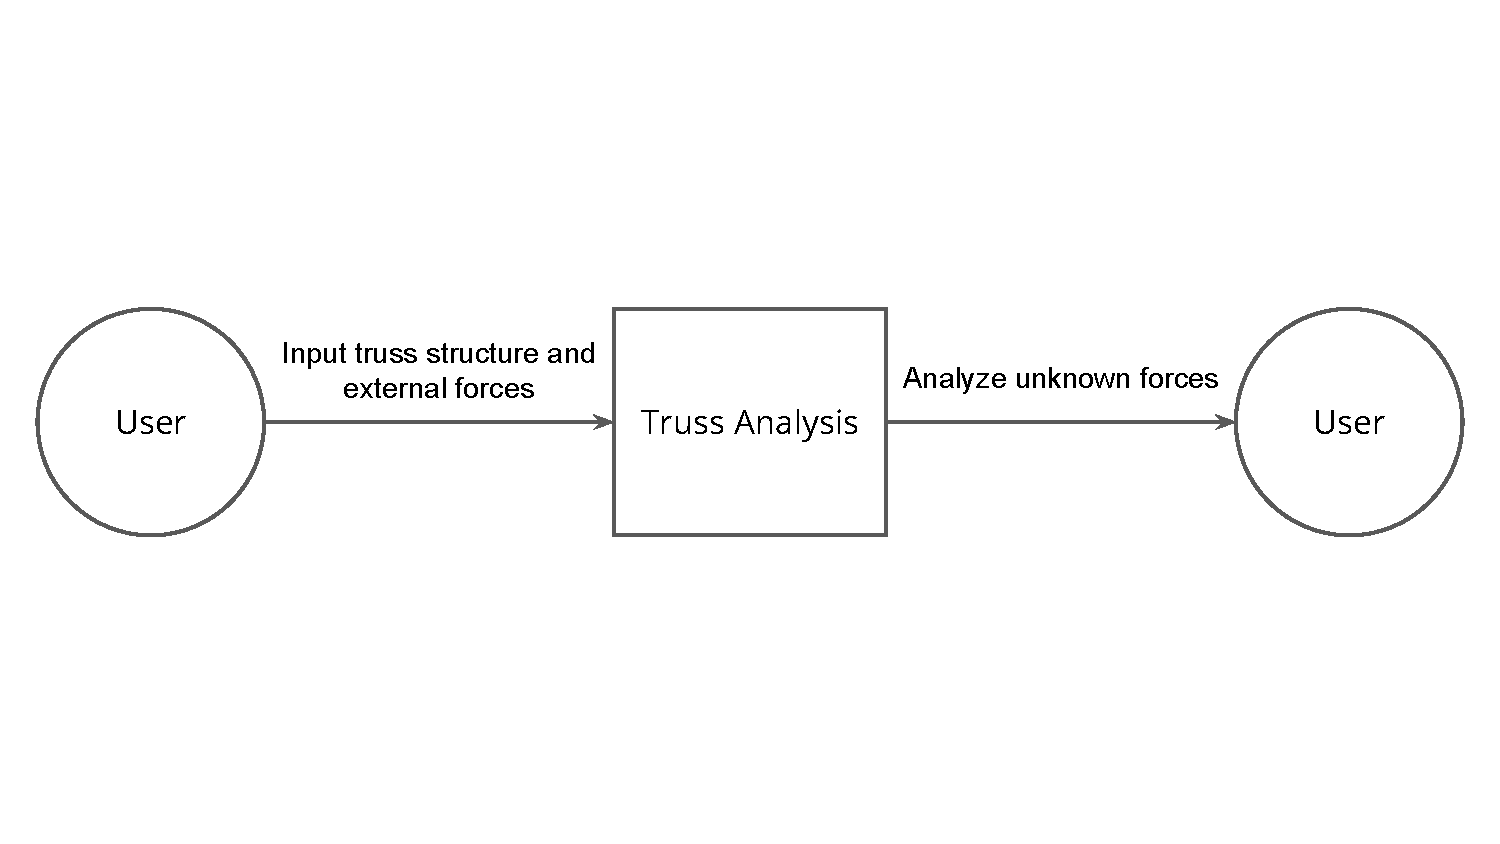
\includegraphics[width=0.6\textwidth]{SystemContext}
\caption{System Context}
\label{Fig_SystemContext} 
\end{center}
\end{figure}

The interaction between the product and the user is through a user interface. 
The responsibilities of the user and the system are as follows:

\begin{itemize}
\item User Responsibilities:
\begin{itemize}
\item Provide the input data to the system, ensuring no errors in the data 
entry.
\item Ensure that the input data is sufficient to specify a truss structure 
that has a unique solution.
\end{itemize}
\item Truss Responsibilities:
\begin{itemize}
\item Detect data type mismatch, such as a string of characters instead of a
  floating point number.
\item Determine if the inputs satisfy the required physical and software 
constraints.
\item Solve the equilibrium equations arising from the input data to generate 
the output data.
\end{itemize}
\end{itemize}

\subsection{User Characteristics} \label{SecUserCharacteristics}
The end user of the system should have an understanding of solving equilibrium 
forces and moments from level 1 engineering mechanic. The system might be used 
as an educational tool for students studying in engineering to master the 
concepts of static equilibrium and truss analysis.

\subsection{System Constraints}
There are no system constraints.

\section{Specific System Description}

This section first presents the problem desciption (Section \ref{Sec_pd}), 
which gives a high-level view of the problem to be solved.  This is followed by 
the solution characteristics specification (Section \ref{Sec_solcharspec}), 
which presents the assumptions, theories, definitions and finally the instance 
models.  

\subsection{Problem Description} \label{Sec_pd}

A system is intended to analyze the unknown forces acting on truss members.

\subsubsection{Terminology and  Definitions}

This subsection provides a list of terms that are used in the subsequent
sections and their meaning, with the purpose of reducing ambiguity and making it
easier to correctly understand the requirements:

\begin{itemize}
	
	\item Compression: the force that squeezes materials together.
	
\end{itemize}

\begin{itemize}
	
	\item Force equilibrium: a body is in force equilibrium if the sum of all 
	the forces acting on the body is zero. 
	
\end{itemize}

\begin{itemize}
	
	\item Joint: a place where two trusses are connected.
	
\end{itemize}

\begin{itemize}
	
	\item Method of Joint: a way to find unknown forces in a truss structure. 
	The principle behind this method is that all forces acting on a joint must 
	add to zero.
	
\end{itemize}

\begin{itemize}
	
	\item Moment: moment of a force, also called \textit{torque}, is the 
	tendency to cause a body to rotate about a 	specific point or axis. 
	
\end{itemize}

\begin{itemize}
	
	\item Moment equilibrium: a body is in moment equilibrium if the sum of all 
	the moments of all the forces acting on the body is zero.
	
\end{itemize}

\begin{itemize}

\item Pin support: a kind of structural support can have both a horizontal x 
direction force and a vertical y direction force.

\end{itemize}

\begin{itemize}
	
	\item Reaction force: an external force on a body which is contributed by 
	its supports or connections.
	
\end{itemize}

\begin{itemize}
	
	\item Roller support: a kind of structural support can only have a 
	vertical y direction force.
	
\end{itemize}

\begin{itemize}
	
	\item Tension: the force that pulls materials apart.
	
\end{itemize}

\subsubsection{Physical System Description} \label{sec_phySystDescrip}

The physical system of Truss, as shown in Figure \ref{Fig_PhysicalSystem},
includes the following elements:

\begin{itemize}

\item[PS1:] The pin support ($S_\text{p}$).

\item[PS2:] The roller support ($S_\text{r}$).

\item[PS3:] The joints (A, B, C, and D).

\item[PS4:] Truss members (1, 2, 3, and 4).

\end{itemize}


\begin{figure}[h!]
	\begin{center}
		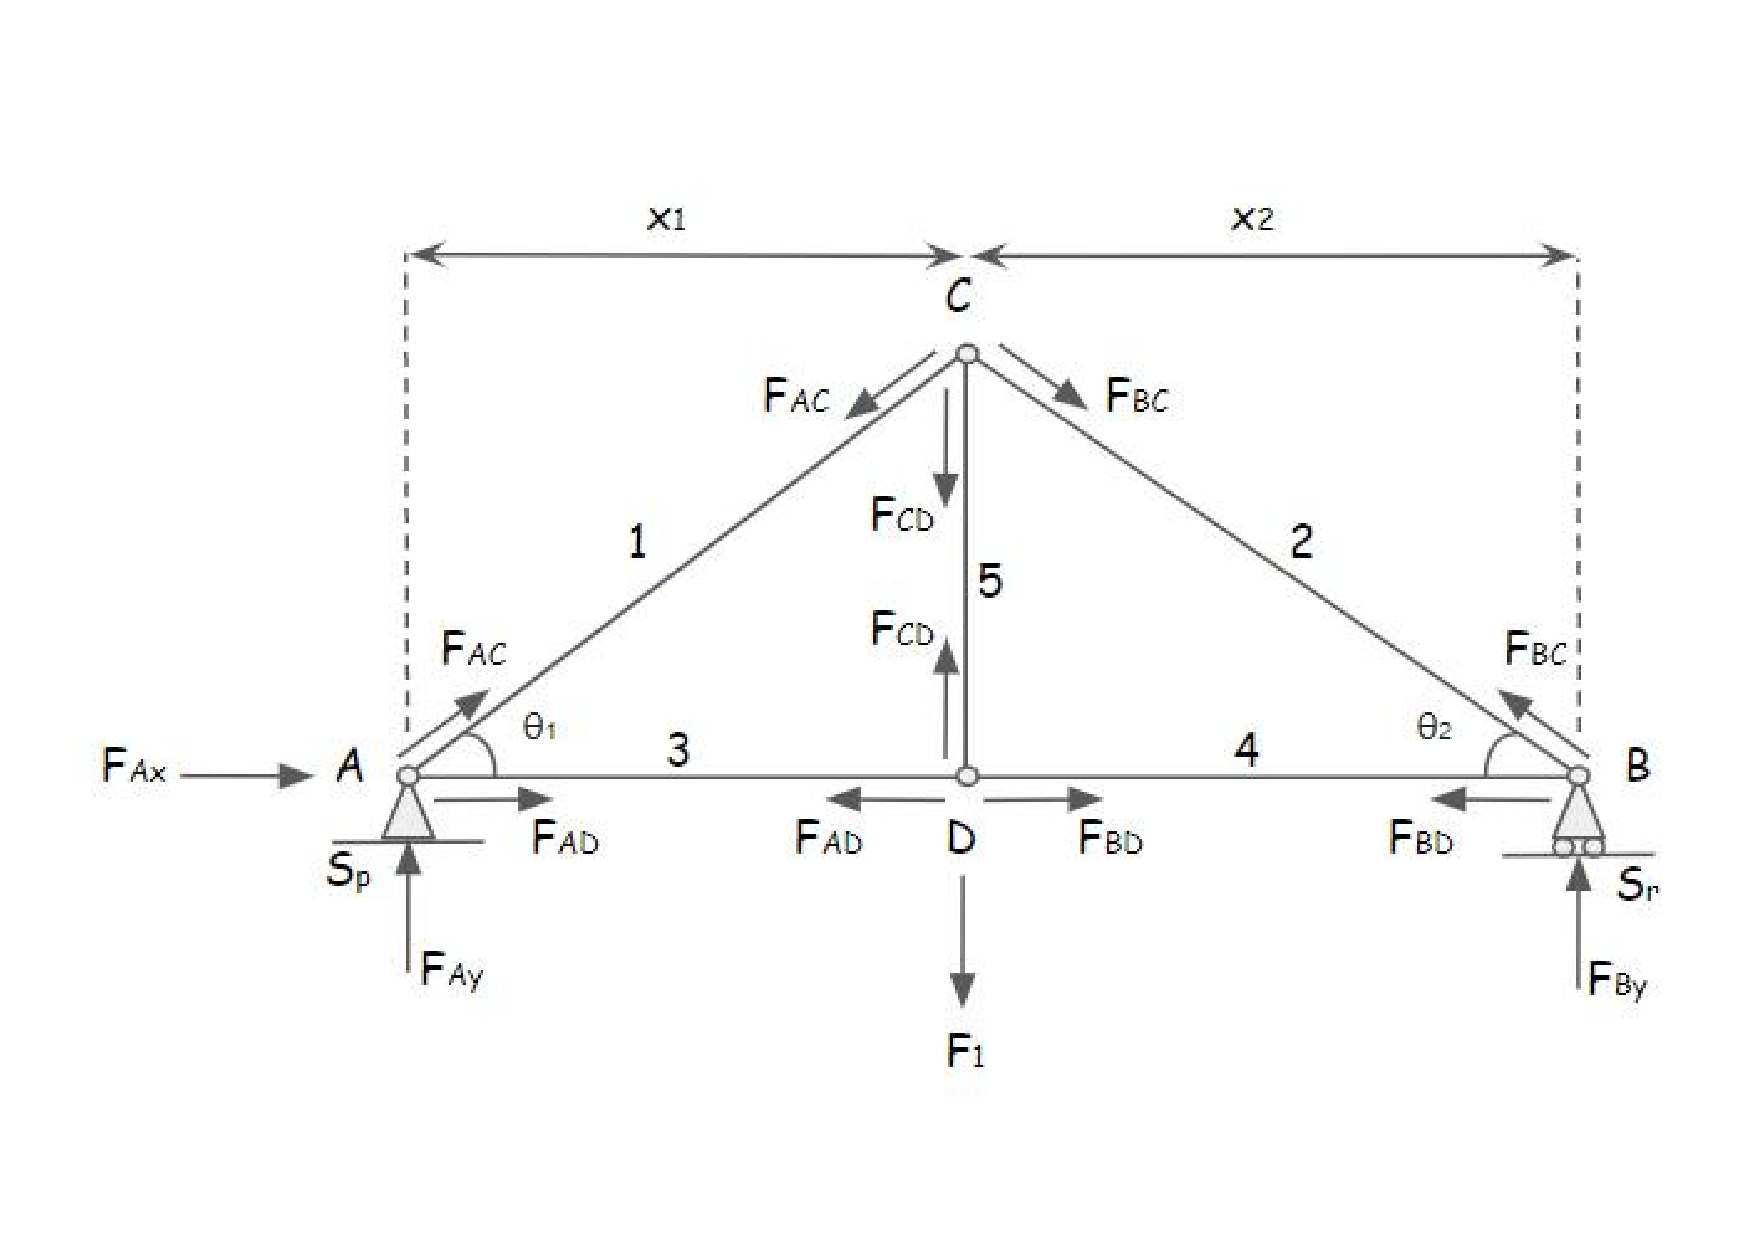
\includegraphics[width=0.6\textwidth]{PhysicalSystem}
		\caption{The physical system}
		\label{Fig_PhysicalSystem} 
	\end{center}
\end{figure}

\subsubsection{Goal Statements}\label{sec_goal}

\noindent 
Given the truss properties and the external force, the goal statement are:

\begin{itemize}
\item[GS\refstepcounter{goalnum}\thegoalnum \label{G_solreactforce}:] 
{Solve the support reaction forces.}

\item[GS\refstepcounter{goalnum}\thegoalnum \label{G_solforce}:] 
{Solve the internal forces acting on truss members.}
\end{itemize}

\subsection{Solution Characteristics Specification} \label{Sec_solcharspec}

The instance models that govern Truss are presented in 
Section~\ref{sec_instance}.  The information to understand the meaning of the
instance models and their derivation is also presented, so that the instance
models can be verified.

\subsubsection{Assumptions} \label{sec_assumpt}

This section simplifies the truss analysis problem in real world and helps in 
developing the theoretical model by filling in the missing information for the 
physical system. The numbers given in the square brackets refer to the 
theoretical model [T], general definition [GD], data definition [DD], instance 
model [IM], or likely change [LC], in which the respective assumption is used.

\begin{itemize}
	
\item[A\refstepcounter{assumpnum}\theassumpnum \label{A_static}:]
 The structure is statically determinate. [\tref{T_staticeq}]
 
\end{itemize}

\begin{itemize}
	
	\item[A\refstepcounter{assumpnum}\theassumpnum \label{A_frictionless}:]
	All joints are connected by frictionless pins. [\lcref{LC_notpinconnect}]
	
\end{itemize}

\begin{itemize}
	
	\item[A\refstepcounter{assumpnum}\theassumpnum \label{A_connectatend}:]
	Truss members are connected only at their end. 
	
\end{itemize}

\begin{itemize}
	
	\item[A\refstepcounter{assumpnum}\theassumpnum \label{A_straight}:]
	All the truss members are perfectly straight. 
	
\end{itemize}

\begin{itemize}
	
	\item[A\refstepcounter{assumpnum}\theassumpnum \label{A_weightig}:]
	The weight of the members are negligibly small which can be ignored. 
	[\lcref{LC_weightinclude}]
	
\end{itemize}

\begin{itemize}
	
	\item[A\refstepcounter{assumpnum}\theassumpnum \label{A_twoforce}:]
	All the members have only tension or compression forces. 
	[\lcref{LC_otherforce}]
	
\end{itemize}

\begin{itemize}
	
	\item[A\refstepcounter{assumpnum}\theassumpnum \label{A_reactionjoint}:]
	All loads and support reactions are applied at the joints only.  
	
\end{itemize}

\subsubsection{Theoretical Models}\label{sec_theoretical}

This section focuses on the general equations and laws that Truss is based
on.  
~\newline

\noindent
\begin{minipage}{\textwidth}
\renewcommand*{\arraystretch}{1.5}
\begin{tabular}{| p{\colAwidth} | p{\colBwidth}|}
  \hline
  \rowcolor[gray]{0.9}
  Number& TM\refstepcounter{theorynum}\thetheorynum \label{T_staticeq}\\
  \hline
  Label&\bf Static equilibrium\\
  \hline
  Equation& $\sum F_{\text{xi}} = 0$ \\
  & $\sum F_{\text{yi}} = 0$ \\
  & $\sum M_{\text{i}} = 0$\\
  \hline
  Description  
  & $F_{\text{xi}}$ is the force component in the x direction of joint i.\\
  & $F_{\text{yi}}$ is the force component in the y direction of joint i.\\
  & $M_{\text{i}}$ is the moment component of joint i. \\
  & A truss is considered statically determinate if $\sum M = 0$ at any point, 
  and both $\sum F_{\text{x}} = 0$, $\sum F_{\text{y}} = 0$.\\
  \hline
  Source & \cite{MethodofJoints}, \cite{Moment}\\
  % The above web link should be replaced with a proper citation to a publication
  \hline
  Ref.\ By & \aref{A_static}, \aref{A_weightig}\\
  \hline
\end{tabular}
\end{minipage}\\

~\newline
\subsubsection{General Definitions}\label{sec_gendef}
There are no general definitions.

\subsubsection{Data Definitions}\label{sec_datadef}

There are no data definitions.

\subsubsection{Instance Models} \label{sec_instance}    

This section transforms the problem defined in Section~\ref{Sec_pd} into 
one which is expressed in mathematical terms. It uses concrete symbols defined 
in Section~\ref{sec_datadef} to replace the abstract symbols in the models 
identified in Sections~\ref{sec_theoretical} and~\ref{sec_gendef}.

The goal \gsref{G_solforce} is met by \iref{I_solveA}, \iref{I_solveB}, and 
\iref{I_solveD}.

~\newline

%Instance Model 1

\noindent
\begin{minipage}{\textwidth}
	\renewcommand*{\arraystretch}{1.5}
	\begin{tabular}{| p{\colAwidth} | p{\colBwidth}|}
		\hline
		\rowcolor[gray]{0.9}
		Number& IM\refstepcounter{instnum}\theinstnum \label{I_solveFax}\\
		\hline
		Label& \bf Support reaction force on joint A in the x direction\\
		\hline
		Input& - \\
		\hline
		Output& $F_{\text{{Ax}}}$ \\
		\hline
		Equation& $F_{\text{Ax}} = 0$ \\
		\hline
		Description&$F_{\text{Ax}}$ is the support reaction force on joint A 
		in the x direction (N). \\
		\hline
		Notes& Because joint A is pinned, there is a reacting force in the x 
		direction, $F_{\text{Ax}}$. We apply the static equilibrium $\sum 
		F_{\text{x}} = 0$ to solve the reaction force. \\
		\hline
		Sources& - \\
		\hline
		Ref.\ By & \aref{A_static}, \aref{A_frictionless}, \aref{A_weightig}, 
		\tref{T_staticeq} \\
		\hline
	\end{tabular}
\end{minipage}\\

~\newline

\noindent
\begin{minipage}{\textwidth}
	\renewcommand*{\arraystretch}{1.5}
	\begin{tabular}{| p{\colAwidth} | p{\colBwidth}|}
		\hline
		\rowcolor[gray]{0.9}
		Number& IM\refstepcounter{instnum}\theinstnum \label{I_solveFay}\\
		\hline
		Label& \bf Support reaction force on joint A in the y direction\\
		\hline
		Input& $F_\text{1}$, $x_\text{1}$, $x_\text{2}$ \\
		\hline
		Output& $F_{\text{{Ay}}}$ \\
		\hline
		Equation& $F_{\text{Ay}} = F_\text{1} \cdot x_\text{2} / (x_\text{1} + 
		x_\text{2})$ \\
		\hline
		Description&$F_{\text{Ay}}$ is the support reaction force on joint A 
		in the y direction (N).\\
		&$F_1$ is the given external force (N).\\
		&$x_1$ is the distance between joint A and joint D (m).\\
		&$x_2$ is the distance between joint D and joint B (m).\\
		\hline
		Notes& We apply the static equilibrium $\sum M_{\text{B}} = F_\text{1} 
		\cdot x_\text{2} - F_{\text{Ay}} \cdot (x_\text{1} + x_\text{2}) = 0$ 
		to solve the reaction force. \\
		&$x_1$ and $x_2$ are shown in figure \ref{Fig_PhysicalSystem}.\\
		\hline
		Sources& - \\
		\hline
		Ref.\ By & \aref{A_static}, \aref{A_frictionless}, \aref{A_weightig}, 
		\tref{T_staticeq} \\
		\hline
	\end{tabular}
\end{minipage}\\

~\newline

\noindent
\begin{minipage}{\textwidth}
	\renewcommand*{\arraystretch}{1.5}
	\begin{tabular}{| p{\colAwidth} | p{\colBwidth}|}
		\hline
		\rowcolor[gray]{0.9}
		Number& IM\refstepcounter{instnum}\theinstnum \label{I_solveFby}\\
		\hline
		Label& \bf Support reaction force on joint B in the y direction\\
		\hline
		Input& $F_\text{1}$, $x_\text{1}$, $x_\text{2}$ \\
		\hline
		Output& $F_{\text{{By}}}$ \\
		\hline
		Equation& $F_{\text{By}} = F_\text{1} \cdot x_\text{1} / (x_\text{1} + 
		x_\text{2})$ \\
		\hline
		Description&$F_{\text{By}}$ is the support reaction force on joint B in 
		the y direction (N).\\
		&$F_1$ is the given external force (N).\\
		&$x_1$ is the distance between point A and point D (m).\\
		&$x_2$ is the distance between point D and point B (m).\\
		\hline
		Notes& We apply the static equilibrium $\sum M_{\text{A}} = 
		F_{\text{By}} \cdot (x_\text{1} + x_\text{2}) - F_\text{1} \cdot 
		x_\text{1} = 0$ to solve the reaction force. \\
		&$x_1$ and $x_2$ are shown in figure \ref{Fig_PhysicalSystem}. \\
		\hline
		Sources& - \\
		\hline
		Ref.\ By & \aref{A_static}, \aref{A_frictionless}, \aref{A_weightig}, 
		\tref{T_staticeq} \\
		\hline
	\end{tabular}
\end{minipage}\\

~\newline

\noindent
\begin{minipage}{\textwidth}
	\renewcommand*{\arraystretch}{1.5}
	\begin{tabular}{| p{\colAwidth} | p{\colBwidth}|}
		\hline
		\rowcolor[gray]{0.9}
		Number& IM\refstepcounter{instnum}\theinstnum \label{I_solveA}\\
		\hline
		Label& \bf Solving for internal forces at point A\\
		\hline
		Input& $F_{\text{Ay}}$, $\theta_1$\\
		\hline
		Output& $F_{\text{{AC}}}$, $F_{\text{{AD}}}$ \\
		\hline
		Equation& $F_{\text{{AC}}} = -F_{\text{Ay}} /$ sin $\theta_1$ \\
		&$F_{\text{{AD}}} = -F_{\text{{AC}}} \cdot$ cos $\theta_1$ \\
		\hline
		Description&$F_{\text{{AC}}}$ is the force in truss 1 (N).\\
		&$F_{\text{{AD}}}$ is the force in truss 3 (N).\\
		&$F_{\text{Ay}}$ is the support reaction force at point A in the y 
		direction (N).\\		
		&$\theta_1$ is the angle between truss 1 and truss 3 (\si{\radian}).\\
		&Truss structure are shown in figure \ref{Fig_PhysicalSystem}.\\
		\hline
		Notes& $\sum F_{\text{y}} = F_{\text{Ay}} + F_{\text{{AC}}} \cdot$ sin 
		$\theta_1 = 0$\\
		&$\sum F_{\text{x}} = F_{\text{AD}} + F_{\text{{AC}}} \cdot$ cos 
		$\theta_1 = 0$\\
		\hline
		Sources& - \\
		\hline
		Ref.\ By & \aref{A_static}, \aref{A_twoforce}, \aref{A_reactionjoint}, 
		\tref{T_staticeq}, \iref{I_solveFay} \\
		\hline
	\end{tabular}
\end{minipage}\\

~\newline

\noindent
\begin{minipage}{\textwidth}
	\renewcommand*{\arraystretch}{1.5}
	\begin{tabular}{| p{\colAwidth} | p{\colBwidth}|}
		\hline
		\rowcolor[gray]{0.9}
		Number& IM\refstepcounter{instnum}\theinstnum \label{I_solveB}\\
		\hline
		Label& \bf Solving for internal forces at point B\\
		\hline
		Input& $F_{\text{By}}$, $\theta_2$\\
		\hline
		Output& $F_{\text{{BC}}}$, $F_{\text{{BD}}}$\\
		\hline
		Equation& $F_{\text{{BC}}} = -F_{\text{By}} /$ sin $\theta_2$ \\
		&$F_{\text{{BD}}} = -F_{\text{{BC}}} \cdot$ cos $\theta_2$ \\
		\hline
		Description&$F_{\text{{BC}}}$ is the force in truss 2 (N).\\
		&$F_{\text{{BD}}}$ is the force in truss 4 (N).\\
		&$F_{\text{By}}$ is the support reaction force at point B in the y 
		direction (N).\\	
		&$\theta_2$ is the angle between truss 2 and truss 4 (\si{\radian}).\\
		&Truss structure are shown in figure \ref{Fig_PhysicalSystem}.\\
		\hline
		Notes& $\sum F_{\text{y}} = F_{\text{By}} + F_{\text{{BC}}} \cdot$ sin 
		$\theta_2 = 0$\\
		&$\sum F_{\text{x}} = F_{\text{BD}} + F_{\text{{BC}}} \cdot$ cos 
		$\theta_2 = 0$\\
		\hline
		Sources& - \\
		\hline
		Ref.\ By & \aref{A_static}, \aref{A_twoforce}, \aref{A_reactionjoint}, 
		\tref{T_staticeq}, \iref{I_solveFby}\\
		\hline
	\end{tabular}
\end{minipage}\\

~\newline

\noindent
\begin{minipage}{\textwidth}
	\renewcommand*{\arraystretch}{1.5}
	\begin{tabular}{| p{\colAwidth} | p{\colBwidth}|}
		\hline
		\rowcolor[gray]{0.9}
		Number& IM\refstepcounter{instnum}\theinstnum \label{I_solveD}\\
		\hline
		Label& \bf Solving for internal forces at point D\\
		\hline
		Input& $F_1$\\
		\hline
		Output& $F_{\text{{CD}}}$ \\
		\hline
		Equation&$F_{\text{{CD}}} = F_1$ \\
		\hline
		Description&$F_{\text{{CD}}}$ is the force in truss 5 (N).\\
		&$F_1$ is the given external force (N).\\
		&Truss structure are shown in figure \ref{Fig_PhysicalSystem}.\\
		\hline
		Notes& $\sum F_{\text{y}} = F_{\text{CD}} - F_1 = 0$\\
		\hline
		Sources& - \\
		\hline
		Ref.\ By & \aref{A_static}, \aref{A_twoforce}, \aref{A_reactionjoint}, 
		\tref{T_staticeq}\\
		\hline
	\end{tabular}
\end{minipage}\\
%~\newline

\subsubsection{Data Constraints} \label{sec_DataConstraints}    

Table~\ref{TblInputCon} shows the data constraints on the input variables.  The 
column for physical constraints gives the physical limitations on the range of 
values that can be taken by the variable. The column for software constraints 
restricts the range of inputs to reasonable values. The software constraints 
will be helpful in the design stage for picking suitable algorithms. The 
constraints are conservative, to give the user of the model the flexibility to 
experiment with unusual situations. The column of typical values is intended to 
provide a feel for a common scenario. The uncertainty column provides an 
estimate of the confidence with which the physical quantities can be measured. 
This information would be part of the input if one were performing an 
uncertainty quantification exercise.

\begin{table}[!h]
  \caption{Input Data Constraints} \label{TblInputCon}
  \renewcommand{\arraystretch}{1.2}
\noindent 
\begin{longtable*}{l l l l c} 
  \toprule
  \textbf{Var} & \textbf{Physical Constraints} & \textbf{Software Constraints} &
                             \textbf{Typical Value} & \textbf{Uncertainty}\\
  \midrule 
  $F_{\text{1}}$ & $F_{\text{1}} > 0$ & $F_{\text{min}} \leq F_{\text{1}} \leq 
  F_{\text{max}}$ & 500 \si{\newton} & 10\%  \\
  $x_{\text{1}}$ & $x_{\text{1}} > 0$ & $d_{\text{min}} < x_{\text{1}} \leq 
  d_{\text{max}}$ & 3 \si{\metre} & 10\%  \\
  $x_{\text{2}}$ & $x_{\text{2}} > 0$ & $d_{\text{min}} < x_{\text{2}} \leq 
  d_{\text{max}}$ & 3 \si{\metre} & 10\%  \\
  $\theta_{\text{1}}$ & $0 < \theta_{\text{1}} < \pi $ & $ \theta_{\text{min}} 
  < \theta_{\text{1}} < \theta_{\text{max}}$ & $\frac{\pi}{4}$ \si{\radian} & 
  10\%  \\
  $\theta_{\text{2}}$ & $0 < \theta_{\text{2}} < \pi $ & $\theta_{\text{min}} < 
  \theta_{\text{2}} < \theta_{\text{max}}$ & $\frac{\pi}{4}$ \si{\radian} & 
  10\%  \\
  \bottomrule
 
\end{longtable*}
\end{table}

\noindent 


%\begin{table}[!h]
%\caption{Specification Parameter Values} \label{TblSpecParams}
%\renewcommand{\arraystretch}{1.2}
%\noindent \begin{longtable*}{l l} 
%  \toprule
%  \textbf{Var} & \textbf{Value} \\
%  \midrule 
%  $L_\text{min}$ & 0.1 \si{\metre}\\
%  \bottomrule
%\end{longtable*}
%\end{table} \

\subsubsection{Properties of a Correct Solution} \label{sec_CorrectSolution}

\noindent
Table~\ref{TblOutputVar} shows the data constraints on the output variables. 
The column for physical constraints gives the physical limitations on the range 
of values that can be taken by the variable.

\begin{table}[!h]
\caption{Output Data Constraints} \label{TblOutputVar}
\renewcommand{\arraystretch}{1.2}
\noindent 
\begin{longtable*}{l l} 
  \toprule
  \textbf{Var} & \textbf{Physical Constraints} \\
  \midrule 
  $F_\text{out}$ & $F_\text{out} > 0$  \\
  \bottomrule
\end{longtable*}
\end{table}

\section{Requirements}

This section provides the functional requirements, the business tasks that the
software is expected to complete, and the nonfunctional requirements, the
qualities that the software is expected to exhibit.

\subsection{Functional Requirements}

\noindent \begin{itemize}
	
\item[R\refstepcounter{reqnum}\thereqnum \label{R_Inputs}:] Input the values 
from Table \ref{TblInputVal}.

\item[R\refstepcounter{reqnum}\thereqnum \label{R_InputsCon}:] Check the 
entered input values to ensure that they do not exceed the data constraints
mentioned in Section \ref{sec_DataConstraints}. If any of the input values are 
out of bounds, an error message is displayed and the calculations stop.

\item[R\refstepcounter{reqnum}\thereqnum \label{R_Calculate}:] Calculate 
equilibrium equations on all joints in both the x and y direction via 
\iref{I_solveFax}, \iref{I_solveFay}, and \iref{I_solveFby}.

\item[R\refstepcounter{reqnum}\thereqnum \label{R_Output}:] Output 
$F_\text{{AC}}$ and $F_\text{{AD}}$ via \iref{I_solveA}, 
$F_\text{{BC}}$ and $F_\text{{BD}}$ via \iref{I_solveB}, and
$F_\text{{CD}}$ via \iref{I_solveD}.

\item[R\refstepcounter{reqnum}\thereqnum \label{R_AnalyzeOutput}:] Analyze what 
kind of forces those outputs are from Table~\ref{TblOutputType}.

\begin{table}[!h]
	\caption{Required Inputs} \label{TblInputVal}
	\renewcommand{\arraystretch}{1.2}
	\noindent \begin{longtable*}{l l l l c} 
		\toprule
		\textbf{Symbol} & \textbf{Description} & \textbf{Units} \\
		\midrule 
		$F_{\text{1}}$ & External force & \si{\newton} \\
		$x_{\text{1}}$ & Distance from joint A to joint D & \si{\metre} \\
		$x_{\text{2}}$ & Distance from joint D to joint B & \si{\metre}  \\
		$\theta_{\text{1}}$ & Angle between member 1 and 3 & \si{\radian} \\
		$\theta_{\text{2}}$ & Angle between member 2 and 4 & \si{\radian}  \\
		\bottomrule
		
	\end{longtable*}
\end{table}

\begin{table}[!h]
	\caption{Output Variables} \label{TblOutputType}
	\renewcommand{\arraystretch}{1.2}
	\noindent 
	\begin{longtable*}{l l} 
		\toprule
		\textbf{Value} & \textbf{Stress Distribution} \\
		\midrule 
		$F_\text{out} > 0$ & Tension \\		
		$F_\text{out} < 0$ & Compression \\
		\bottomrule
	\end{longtable*}
\end{table}
\end{itemize}

\subsection{Nonfunctional Requirements}

\noindent 

\begin{itemize}
\item [NFR\refstepcounter{nonreqnum}\thenonreqnum \label{NFR_Accuracy}:] 
\textbf{Accuracy.} The accuracy of the computed solutions should meet the level 
needed 
for structural mechanic and have the properties described in Section 
\ref{sec_CorrectSolution}.
\item [NFR\refstepcounter{nonreqnum}\thenonreqnum \label{NFR_Verifiability}:]
\textbf{Verifiablility.}: The properties of the software should be able to 
tested easily through verification and validation plan 
(\href{https://github.com/tingyuw/cas741/blob/master/docs/VnVPlan/VnVPlan.pdf}{VnV
 Plan}). 
\item [NFR\refstepcounter{nonreqnum}\thenonreqnum 
\label{NFR_Understandability}:]
\textbf{Understandablility.} The source code and the design of the software 
should be understandable by a new developer.
\item [NFR\refstepcounter{nonreqnum}\thenonreqnum \label{NFR_Portability}:] 
\textbf{Portability.} The software is able to run on different environments, 
such as Windows, MacOS, and Linux.
\item [NFR\refstepcounter{nonreqnum}\thenonreqnum \label{NFR_Maintainability}:]
\textbf{Maintainability.} The software can be modified and improved easily.
\item [NFR\refstepcounter{nonreqnum}\thenonreqnum \label{NFR_Reliability}:]  
\textbf{Reliability.} The probability of failure-free software operation 
for required functions for a specified period of time.
\item [NFR\refstepcounter{nonreqnum}\thenonreqnum \label{NFR_Usability}:] 
\textbf{Usability.} The system should be able to learn and use easily for 
users. 

\end{itemize}

\section{Likely Changes}    
This section lists the likely changes to be made to the software.
\noindent \begin{itemize}

\item[LC\refstepcounter{lcnum}\thelcnum\label{LC_notpinconnect}:] Joints may 
not connected by pins. [\aref{A_frictionless}]

\item[LC\refstepcounter{lcnum}\thelcnum\label{LC_weightinclude}:] The 
software may be changed to consider the weight of the trusses.
[\aref{A_weightig}]

\item[LC\refstepcounter{lcnum}\thelcnum\label{LC_otherforce}:] There are other 
forces involved in (e.g., shearing and bending). [\aref{A_twoforce}]

\end{itemize}

\section{Unlikely Changes}    
This section lists the unlikely changes to be made to the software.
\noindent \begin{itemize}

\item[UC\refstepcounter{ucnum}\theucnum\label{UC_sysgoal}:] The goal of the 
system is to find out the internal forces. [\gsref{G_solforce}]

\item[UC\refstepcounter{ucnum}\theucnum\label{UC_static}:] The truss structure 
is statically determinate. [\aref{A_static}]

\item[UC\refstepcounter{ucnum}\theucnum\label{UC_straight}:] The truss members 
are straight. [\aref{A_straight}]

\end{itemize}

\section{Traceability Matrices and Graphs}

The purpose of the traceability matrices is to provide easy references on what
has to be additionally modified if a certain component is changed. Every time a
component is changed, the items in the column of that component that are marked
with an ``X'' may have to be modified as well. Table~\ref{Table:trace} shows 
the dependencies of theoretical models, general definitions, data definitions, 
and instance models  with each other. Table~\ref{Table:R_trace} shows the
dependencies of instance models, requirements, and data constraints on each
other. Table~\ref{Table:A_trace} shows the dependencies of theoretical models,
general definitions, data definitions, instance models, and likely changes on
the assumptions.

\begin{table}[h!]
\centering
\begin{tabular}{|c|c|c|c|c|c|c|c|}
\hline        
	& \tref{T_staticeq}& \iref{I_solveFax}& \iref{I_solveFay}& 
	\iref{I_solveFby} & \iref{I_solveA}& \iref{I_solveB}& \iref{I_solveD} \\
\hline
\tref{T_staticeq} & & & & & & & \\ \hline
\iref{I_solveFax} &X & & & & & & \\ \hline
\iref{I_solveFay} &X & & & & & & \\ \hline
\iref{I_solveFby} &X & & & & & & \\ \hline
\iref{I_solveA}   &X & &X & & & & \\ \hline
\iref{I_solveB}   &X & & &X & & & \\ \hline
\iref{I_solveD}   &X & & & & & & \\ \hline
\end{tabular}
\caption{Traceability Matrix Showing the Connections Between Items of Different Sections}
\label{Table:trace}
\end{table}

\begin{table}[h!]
\centering
\begin{tabular}{|c|c|c|c|c|c|c|c|}
\hline
	& \iref{I_solveFax}& \iref{I_solveFay}& \iref{I_solveFby}& \iref{I_solveA}& 
	\iref{I_solveB}& \iref{I_solveD}& \ref{sec_DataConstraints} \\
\hline
\rref{R_Inputs}       & & & & & & &\\ \hline
\rref{R_InputsCon}    & & & & & & &X\\ \hline
\rref{R_Calculate}    &X &X &X & & & &\\ \hline
\rref{R_Output}       & & & &X &X &X &\\ \hline
\rref{R_AnalyzeOutput}& & & & & & &\\ \hline 
\end{tabular}
\caption{Traceability Matrix Showing the Connections Between Requirements and Instance Models}
\label{Table:R_trace}
\end{table}

\begin{table}[h!]
	\centering
	\begin{tabular}{|c|c|c|c|c|c|c|c|c|c|c|c|c|c|c|c|c|c|c|c|}
		\hline
		& \aref{A_static}& \aref{A_frictionless}& \aref{A_connectatend}& 
		\aref{A_straight}& \aref{A_weightig}& \aref{A_twoforce}& 
		\aref{A_reactionjoint} \\
		\hline
		\tref{T_staticeq}       &X & & & &X & & \\ \hline
		\iref{I_solveFax}       &X &X & & &X & & \\ \hline
		\iref{I_solveFay}       &X &X & & &X & & \\ \hline
		\iref{I_solveFby}       &X &X & & &X & & \\ \hline
		\iref{I_solveA}         &X & & & & &X &X \\ \hline
		\iref{I_solveB}         &X & & & & &X &X \\ \hline
		\iref{I_solveD}         &X & & & & &X &X \\ \hline
		\lcref{LC_notpinconnect}& &X & & & & & \\ \hline
		\lcref{LC_weightinclude}& & & & &X & & \\ \hline
		\lcref{LC_otherforce}   & & & & & &X & \\ \hline
	\end{tabular}
	\caption{Traceability Matrix Showing the Connections Between Assumptions 
	and Other Items}
	\label{Table:A_trace}
\end{table}


\section{Values of Auxiliary Constants}
Table~\ref{TblAuxConst} contains the standard values that are used for 
calculations in Truss.

\begin{table}[h!]
	\renewcommand{\arraystretch}{1.2}
	\noindent \begin{longtable*}{l l l l c} 
		\toprule
		\textbf{Symbol} & \textbf{Description} & \textbf{Value} & 
		\textbf{Units} \\
		\midrule 
		$F_{\text{max}}$ & the maximum value for external force & 100000 & 
		\si{\newton}\\
		$F_{\text{min}}$ & the minimum value for external force & -100000 & 
		\si{\newton}\\
		$d_{\text{max}}$ & the maximum value for distance & 100000 & 
		\si{\metre}\\
		$d_{\text{min}}$ & the minimum value for distance & 0 & 
		\si{\metre}\\
		$\theta_{\text{max}}$ & the maximum value for amgle & 90 & 
		\si{\radian}\\
		$\theta_{\text{min}}$ & the minimum value for angle & 0 & 
		\si{\radian}\\
		\bottomrule		
	\end{longtable*}
	\caption{Auxiliary Constants} \label{TblAuxConst}
\end{table}

\newpage
\clearpage


\bibliographystyle {plainnat}
\bibliography {ref}

\end{document}